%\documentclass[notes, 9pt]{beamer}      % print frame + notes
%\documentclass[notes=only, 9pt]{beamer} % only notes
\documentclass[9pt]{beamer}              % only frames
%\documentclass[handout, 9pt]{beamer}

%pgfpagesuselayout{4 on 1}

% Notes within frame content
% \mode<handout>{\newline\textcolor{red}{notetext}}

\usetheme[progressbar=frametitle]{metropolis}

\usepackage{booktabs}
\usepackage{hyperref}
% \usepackage[scale=2]{ccicons}
\usepackage{xspace}
\newcommand{\themename}{\textbf{\textsc{metropolis}}\xspace}
\usepackage{graphicx}
\usepackage{subfiles}
\usepackage{tikz}
\usepackage[cache=false]{minted}
\usepackage{tcolorbox}
\tcbuselibrary{minted, skins, listings}

\definecolor{cppcodebg}{rgb}{0.20,0.20,0.20} %0.85

\newtcblisting{cppcode}[1][]{
    listing engine=minted,
    colback=cppcodebg,
    colframe=black!70,
    listing only,
    size=tight,
    minted style=scott,
    minted language=cpp,
    minted options={
        breaklines=true,
        fontsize=\footnotesize,
        tabsize=2,
        linenos=true,
        numbersep=2mm,
        texcl=true,
        #1
    },
    left=5mm,
    enhanced,
    overlay={\begin{tcbclipinterior}\fill[black!25] (frame.south west)
            rectangle ([xshift=5mm]frame.north west);\end{tcbclipinterior}}
}

\newtcblisting{commandshell}{
    colback=cppcodebg, %black
    colupper=white,
    colframe=black!70,
    size=small,
    listing only,
    listing options={style=tcblatex, language=sh},
    every listing line={\textcolor{black!60}{\small\ttfamily\bfseries[user@pc]\$ }}
}

%\begin{commandshell}
%    Hello World!
%\end{commandshell}




% -------------------------------------------------------------------
% Title

\title{Lecture 1: Introduction to C++ Programming}
\subtitle{Curtin FIRST Robotics Club (FRC) Pre-season Training}
\date{\today}
\author{Scott Day}
\email{265815F@curtin.edu.au}
\institute{Curtin University}



% -------------------------------------------------------------------
\begin{document}
% -------------------------------------------------------------------

% -------------------------------------------------------------------
% Table of Contents

\maketitle

\begin{frame}[fragile]{Insert Mandatory Programming Joke}
    \begin{center}
        \makebox[\textwidth]{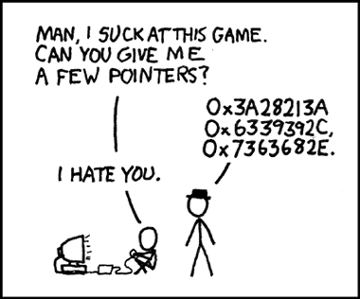
\includegraphics[width=0.95\paperwidth,height=0.95\textheight]{graphics/xkcd138-pointers.png}}
    \end{center}
\end{frame}

\begin{frame}{Table of contents}
  \setbeamertemplate{section in toc}[sections numbered]
  \tableofcontents[hideallsubsections]
\end{frame}

% -------------------------------------------------------------------
% Core

\subfile{sections/programming.tex}
\subfile{sections/cpp.tex}
\subfile{sections/environmentsetup.tex}
\subfile{sections/editingcompilingandexecution.tex}

% -------------------------------------------------------------------
% References

\begin{frame}[allowframebreaks]{References}
    I should fill this out
    \bibliography{sections/references}
    \bibliographystyle{abbrv}
\end{frame}

% http://xkcd.com/138/
% http://xkcd.com/1619/
% http://weknowmemes.com/wp-content/uploads/2012/02/breading-cats-2.jpg
% https://imgs.xkcd.com/comics/goto.png
% http://www.dandelion-films.com/c-programming-memes-17.jpg
% https://xkcd.com/1168/

% -------------------------------------------------------------------
\end{document}
